\cotefile{97}

% H97-01_97_scan019
\scanpage{19}\mspage{- IV- \handwritten{1102} -}
(21.6.5) Considérons donc un diviseur \uline{positif} $D^{\unsure{\prime}}$ sur $X$\inserted{ ($X$ é\deleted{\unsure{n}}tant supposé \uline{noethérien})}, de sorte que l'Idéal \inserted{fractionnaire} $\underline I_{X}(D)$ est un \uline{Idéal de} $\underline O_{X}$, qui est un $\underline O_{X}$-Module \uline{inversible}; soit $Y(D)$ le sous-préschéma fermé de $X$ qu'il définit. \deleted{\unsure{Cela signifie}}\inserted{Pour} \deleted{\unsure{qu}} tout $x\handwritten{\in}Y(D)$, \deleted{\unsure{que,}} il y a par hypothèse un voisinage \inserted{\handwritten{ouvert}} $U$ de $x$ dans $X$ et une section \uline{régulière} $t\handwritten{\in\Gamma}(U,\underline O_{X})$ telle que $\underline I_{X}(D)\handwritten{\mid}U=\underline O_{U}\mathbin{.}t$ (21.2.7) ; en d'autres termes, l'immersion canonique $Y(D)\handwritten{\to}X$ est \uline{régulière et de codimension 1} \inserted{(19.1.4) en tout point de $Y( D)$}. On notera d'ailleurs qu'inversement, si $Y$ \reversemarginpar
% slanted
\margin{\figure{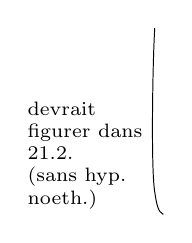
\begin{tikzpicture}[x=1em,y=1em,baseline=0pt]
  \node[anchor=north east,align=left,inner sep=0pt,font=\scriptsize] at (0,0)
    {\handwritten{devrait}\\
     \handwritten{figurer dans}\\
     \handwritten{21.2.}\\
     \handwritten{(sans hyp.}\\
     \handwritten{noeth.)}};
  \draw[line width=.35pt] (.43,2.65) .. controls (.36,1.6) and (.29,-2.25) .. (.42,-3.2)
     .. controls (.49,-3.7) and (.55,-4) .. (.74,-4.08);
\end{tikzpicture}}}
est un sous-préschéma fermé de $X$, régulièrement immergé dans $X$ et \deleted{\unsure{est}} de codimension $1$ en tout point de $Y$, il existe un diviseur positif et un seul \deleted{\unsure{positif}} $D$ sur $X$ tel que $Y(D)=Y$, car\deleted{\unsure{ cela signifie}}\inserted{ pour} \deleted{\unsure{qu}} tout $x\handwritten{\in}Y$, il y a un voisinage $U$ de $x$ dans $X$ tel que $Y\handwritten{\cap}U$ soit défini par un Idéal de $\underline{\mathbb{O}}_{U}$ de la forme $\underline O_{U}\mathbin{.}t$, où $t$ est \uline{réguli\deleted{\unsure{re}}\handwritten{er}} dans $\handwritten{\Gamma}(U,\underline O_{X})$.


Puisque $X$ est supposé noethérien, $Y(D)$ n'a qu'un nombre fini de points maximaux, et en chacun de ces points $x$, on a $\operatorname{codim}(\handwritten{\{}x\handwritten{\}},X)={}\allowbreak{}=\operatorname{dim}(\underline O_{X,x})=1$, autrement dit $x\handwritten{\in}X^{(1)}$ ;
% slanted
\margin{\handwritten{\uline{réf} !}}\normalmarginpar
\deleted{\illegible{2} \unsure{partie} \illegible{1}} en outre, $\underline O_{Y(D),x}$ est un anneau \uline{artinien} en chacun de ces poi\deleted{g}nts. En tout point $x\handwritten{\in}X^{(1)}$ qui n'est pas point maximal de $Y(D)$, on a nécessairement $x\handwritten{\notin}Y(D)$, donc $\underline O_{Y(D),x}=0$. Posons
\[
  \operatorname{cyc}(D)=\handwritten{\sum}^{\handwritten{\prime}}_{x\handwritten{\in}X^{(1)}}
  \operatorname{long}(\underline O_{Y(D),x})\mathbin{.}\handwritten{\overline}{\handwritten{\{}x\handwritten{\}}}
  \tag*{(21.6.5.1)}
\]
qui est donc un élément de $Z^{1}(X)$.

\uline{Proposition} (21.6.6) .- \deleted{\uline{Si} $X$ \uline{est noethérien}}, \uline{\deleted{l}\handwritten{L}'application} $D\handwritten{\leadsto}\operatorname{cyc}(D)$\deleted{\unsure{;}} \uline{est un homomorphisme du monoïde} $\operatorname{Div}^{+}(X)$ \uline{dans} $Z^{1}(X)$ .

Tout revient à voir que pour deux diviseurs \uline{positifs} $D,D'$, on a $\operatorname{cyc}(D+D')=\operatorname{cyc}(D)+\operatorname{cyc}(D')$. Or, on a (21.2.5) $\underline I_{X}(D+D')=\underline I_{X}(D)\underline I_{X}(D')$; tout revient à voir que si $x\handwritten{\in}X^{(1)}$, \inserted{\handwritten{si l'on pose}} $A=\underline O_{X,x}$, et si $t$ et $t'$ sont deux éléments réguliers de $A$, on a $\operatorname{long}(A/tt'A)=\operatorname{long}(A/tA)+{}\allowbreak{}+\operatorname{long}(A/t'A)$ ; mais puisque \deleted{\unsure{$x$}} $t$ est régulier, $tA/tt'A$ est isomorphe à $A/t'A$, d'où \deleted{\unsure{résulte}} aussitôt la proposition.

Il résulte aussitôt des définitions que pour tout ouvert $U\handwritten{\subset}X$, on
% archive sheet number: 18

\cotefile{123}

% C123-01_123_scan002
\scanpage{2}
Compléments sur transformation de Coxeter d'un système de racines\inserted{\handwritten{irréductible}} (Kostant).
\margin{\handwritten{The principal 3-dimensional subgroup ....\quad th. 9.2.}}
% The insertion above the title is enclosed in an oval, with a leader to after ``racines''.
\margin{\handwritten{\figure{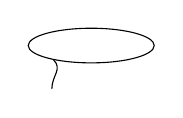
\begin{tikzpicture}[x=1cm,y=1cm]\draw (0,0) ellipse (0.8 and 0.22);\draw (-0.48,-0.18) .. controls (-0.36,-0.3) and (-0.5,-0.38) .. (-0.5,-0.55);\end{tikzpicture}}}}

a) Soit $w\handwritten{\in}W$. Alors toute valeur propre de $w$ \deleted{\unsure{di}}est une racine de $1$ d'ordre divisant un des entiers $m_i+1$ (où les $m_i$ sont les exposants caractéristiques), donc d'ordre $\handwritten{\leq}h$. Pour qu'il y en ait une qui soit d'ordre $h$, il faut et suffit que $w$ soit une transformation de Coxeter, et\inserted{alors} les éléments non nuls du sous-espace propre correspondant\handwritten{\tikz[baseline=.1ex,x=1em,y=1em]{\draw (0,0) circle (.13);\draw (.09,.1)--(.72,.9);}}\inserted{\handwritten{(qui est de dim $1$)}} sont des éléments réguliers.
% A right marginal bracket holds the paragraph a).
\margin{\handwritten{\figure{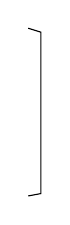
\begin{tikzpicture}[x=1cm,y=1cm]\draw (-0.16,0.05)--(0,0)--(0,-2.05)--(-0.16,-2.08);\end{tikzpicture}}}}

\uline{Corollaire}\handwritten{1}: Soit $\handwritten{\mu}$ le sous-groupe de $W$ engendré par un élément de Coxeter $c$, donc $\handwritten{\mu\simeq}\underline{Z}\handwritten{/}h\underline{Z}$. Alors $\handwritten{\mu}$ est égal au centralisateur de $c$, donc de $\handwritten{\mu}$, et si $\handwritten{\nu}$ est le normalisateur de $\handwritten{\mu}$, l'homomorphisme
% A left marginal rule holds the corollary through ``mod mu''.
\margin{\handwritten{\figure{\begin{tikzpicture}[x=1cm,y=1cm]\draw (0,0)--(0,-2.4);\end{tikzpicture}}}}
\[
\handwritten{\unsure{\psi|\nu}/\mu\longrightarrow}\operatorname{Aut}(\handwritten{\mu})\handwritten{\simeq}(\underline{Z}/h\underline{Z})^{\handwritten{*}}
\]
\margin{\handwritten{Quelle extension de $(\unsure{Z|\mathbb{Z}}/hZ]^{*}$ par $Z/hZ$ obtient-on ?}}
est u\deleted{j}n isomorphisme; en d'autres termes, pour tout entier $n$ premier à $h$, il existe un $w\handwritten{\in}W$ tel que $wcw^{-1}=c^h$, et $w$ est déterminé mod $\handwritten{\mu}$.
\margin{\handwritten{\unsure{échanger|échange} avec cor.\unsure{3|?}}}

Soit \deleted{\unsure{D|B}}en ef\inserted{\handwritten{f}}et $D$ \deleted{\unsure{une droite}}\inserted{le sous-espace} propre sous $c$ correspondant à une racine primitive $h$.ème de $1$. Alors $\dim D=1$ (prop.30), et $\handwritten{\mathfrak{z}}=\operatorname{Centr}(\handwritten{\mu})$ normalise $D$, d'où un homomorphisme $\handwritten{\mathfrak{z}\to}\operatorname{Aut}(D)=\underline{C}^{\handwritten{*}}$, dont l'image est un sous-groupe fini de $\underline{C}^{\handwritten{*}}$, contenant l'image (isomorphe) de $\handwritten{\mu}$, donc cyclique d'ordre un multiple de $h$. Grâce à Kostant, son ordre est égal à $h$, et on a donc trouvé une rétraction $\handwritten{\mathfrak{z}\to\mu}$, il faut prouver que son noyau est réduit à $1$. Or si $w$ est dans ce noyau, il \deleted{induit} centralise $D$, et \unsure{qômme|qomme} $D$ est régulière par Kostant,cela implique $w=1$. \deleted{\unsure{B}}On a donc prouvé $\handwritten{\mathfrak{z}}=\handwritten{\mu}$. Reste à prouver que si $n$ est un entier premier à $h$, alors $c^n$ est conjugué de $c$, ce qui résulte également de Kostant.

\uline{Coroll\deleted{b}a\deleted{\unsure{j|l}}ire}. Soit $c$ un élément de Coxeter, et $\handwritten{\lambda}$ une valeur propre de $c$, correspondant à un vecteur propre $x$. Pour que $x$ soit régulier, il faut et il suffit que $\handwritten{\lambda}$ soit une racine primitive $h$.ème de $1$.
% A left marginal rule holds this corollary.
\margin{\handwritten{\figure{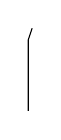
\begin{tikzpicture}[x=1cm,y=1cm]\draw (0.05,0)--(0,-0.15)--(0,-1.05);\end{tikzpicture}}}}

La suffisance a déjà été énoncée avec le th. de Kostant. Pour la nécessité, soit $h'\handwritten{\leq}h$ l'ordre de la valeur propre, alors $c^{h'}$ centralise $x$, donc, $x$ étant régulier, on a $c^{h'}=1$, donc $h'=h$, cqfd.

\uline{Corollaire}. \deleted{\unsure{Considérons}} \deleted{Soit $D$ une}\inserted{Soit $D$ une} droite régulières dans $V\otimes\underline{C}$ telle qu'il existe un élé%
% archive sheet number: 1

% C123-01_123_scan003
\scanpage{3}ment de Coxeter\inserted{\handwritten{$c$}} de $W$ qui la normalise. Alors le normalisateur de $\deleted{W}D$ dans $W$ est le groupe engendré par $c$, et il existe une unique élément de Coxeter de $W$ normalisant $D$ et y ayant pour valeur propre une racine \deleted{de}primitive \unsure{\inserted{$h$.ème}} donnée de $1$. Les droites régulières $D$ ayant la propriété précédente (appelées ``droites cycliques'' par Kostant) sont conjuguées sous $W$, leur nombre est égal à $\operatorname{card}(W)/h$.

NB Dans l'ensemble des droites cycliques, le groupe $(\underline{Z}/h\underline{Z})^{\handwritten{*}}$ opère\inserted{en commutant à l'action de $W$} librement; deux droites cycliques sont conjuguées sous l'action de ce groupe si et seulement si elles ont même stabilisateur dans $W$.
% archive sheet number: 2

% C123-01_123_scan016
\scanpage{16}
Résumé de quelques résultats de Kostant (sous groupes simples de rang $1$).

$G$ est un groupe semi-simple sur un corps $k$ de car. nulle, $\handwritten{\mathfrak{g}}$ son algèbre de Lie,
\margin{\handwritten{(The principal 3-dimensional subgroup...., Am. Jour. Oct.1959, 3.4, 3.5, 3.6, \unsure{1.2|4.2}, 9.3)}}

\uline{Théorème} 1. \inserted{\handwritten{(i)}} Soi\deleted{\unsure{t}}ent $x,e\handwritten{\in\mathfrak{g}}$,\inserted{avec $e\handwritten{\ne}0$, $e$ nilpotent.} Pour tout entier $k$, soit $\handwritten{\mathfrak{g}}(k)$ le sous-espace propre de\hspace{1.5em} correspondant à la valeur propre $k$. Donc si $x=\operatorname{Lie}(i)(1)$, où $i:\underline{G}_m\handwritten{\longrightarrow}G$, les $\handwritten{\mathfrak{g}}(k)$ sont les \deleted{décomposition} composants de $\handwritten{\mathfrak{g}}$ suivant les caractères de $\underline{G}_m$, opérant sur $\handwritten{\mathfrak{g}}$ via $i$ et la représentation adjointe. Les conditions suivantes sont équiva\deleted{\unsure{e}}lentes:

\[
\text{a)}\quad e\handwritten{\in\mathfrak{g}}(2)\quad\text{i.e.}\quad \handwritten{[}x,e\handwritten{]}=2e,\quad\text{et }\inserted{\text{pour tout entier }k\handwritten{\geq}1,}\quad\operatorname{ad}(e)^k:\handwritten{\mathfrak{g}}(-k)\handwritten{\longrightarrow\mathfrak{g}}(k)\quad\text{est un isom.}
\]

\[
\text{b)}\quad e\handwritten{\in\mathfrak{g}}(2),\quad\handwritten{\deleted{\unsure{et}}}\quad \operatorname{ad}(e):\handwritten{\mathfrak{g}}(0)\handwritten{\longrightarrow\mathfrak{g}}(-2)\quad\text{est surjectif},
\]
\inserted{\handwritten{et $x$ est de la forme $f(x_o)$, pour $f:\operatorname{Sl}(2,k)\to G$ (\uline{élément de Dynkin}).}}

\handwritten{\deleted{b') Comme b), avec $\operatorname{ad}(e):\mathfrak{g}(0)\to\mathfrak{g}(\unsure{2|-2})$ \uline{\unsure{bijectif}}}}

\[
\text{c)}\quad e\handwritten{\in\mathfrak{g}}(2),\quad\text{et }x\handwritten{\in}\operatorname{ad}(e)(\handwritten{\mathfrak{g}}).
\]

\[
\text{c')}\quad e\handwritten{\in\mathfrak{g}}(2),\quad\text{et }x\handwritten{\in}\operatorname{ad}(e)(\handwritten{\mathfrak{g}}(-2)).
\]

d) Il existe un homomorphisme $f:\operatorname{Sl}(2,k)\handwritten{\longrightarrow}G$ tel que $f^{\handwritten{'}}(e_o)=e,f^{\handwritten{'}}(x_o)=x\deleted{y}$ où $(x_o,e_o,f_o)$ est la base de $\operatorname{Lie}\operatorname{Sl}(2,k)$ correspondant à l'épinglage habituel de ce groupe.

C$\overset{-}{\underset{\text{\unsure{e}}}{\text{e}}}$s conditions impliquent qu'i\deleted{\unsure{o|b}}l existe un homomorphisme $i:\underline{G}_m\handwritten{\longrightarrow}G$, tel que $\operatorname{Lie}(i)(1)=x$, a fortiori que $x$ est semi-simple. De plus, le $f$ de d) est déterminé de façon unique.

(ii) Pour tout élément nilpotent $e$ de $\handwritten{\mathfrak{g}}$, il existe un homomorphisme $f:\operatorname{Sl}(2,k)\handwritten{\longrightarrow}G$ tel que $f(e_o)=e$, ou ce qui revient au même, tel que $f(u_o)=u$ (où $u=\exp(e)$, $u_o=\exp(e_o)$);\inserted{\handwritten{$f$ est uniquement déterminé \unsure{par} $x=f(x_o)$ i.e., par $i=f\circ i_o$.}} \deleted{\unsure{e}}\handwritten{E}n vertu de (i), il revient au même,\deleted{\unsure{(}}lorsque $e=0$ i\handwritten{/}.e. $u\handwritten{\ne}1$, de dire qu'il existe un $x\handwritten{\in\mathfrak{g}}$ tel que $(x,e)$ satisfasse aux conditions équivalentes de (i), ou encore un homomorphisme $i:\underline{G}_m\handwritten{\longrightarrow}G$ tel que $(\operatorname{Lie}(i)(1),e)$ y satisfasse. Les homomorphismes $f$ en question sont conjugués \deleted{sous les éléments de}\inserted{par $\handwritten{Z=}$}$\operatorname{Cent}(e)=\operatorname{Cent}(u)$ (i.e. pour $e\handwritten{\ne}0$, les $x$ en question, ou encore les $i$ en question, sont conjugués \deleted{sous} par $\operatorname{Cent}(u)$), et lorsque $e\handwritten{\ne}0$, les \deleted{\unsure{morphismes}\quad $g$\quad $\operatorname{int}(g)$} $f$ en question (ou encore les
% archive sheet number: 15

% C123-01_123_scan017
\scanpage{17}
$x$ en question, ou les $i$ en question) forment un \uline{torseur} sous le groupe $\handwritten{Z^+}=$\deleted{$\handwritten{\unsure{U\cap}}\operatorname{Cent}(u)$}\inserted{$\handwritten{Z\cap U}$}, qui est un groupe unipotent\inserted{\handwritten{\deleted{(en fait, $\unsure{\subset|c}U$ introduit dans (iv))}}}\handwritten{.}
\margin{\handwritten{cf plus bas définition de $U$. On a $Z\simeq Z_{\unsure{o|0}}.Z^+$ \deleted{\unsure{Commuté|Commutatif}} (produit semi-direct) avec $Z_o=Z\cap L=\operatorname{Cent}(f)$.}}
Enfin, supposant toujours $e\handwritten{\ne}0$, l'ensemble des $x$ en question est un torseur sous \deleted{$\handwritten{\mathfrak{g}}^{e}=$ (centralisateur de $e$ \deleted{\unsure{dans}} dans $\handwritten{\mathfrak{g}}$)$=\operatorname{Ker}\operatorname{ad}(e)=\operatorname{Lie}\operatorname{Cent}(u)$}\inserted{$\handwritten{\operatorname{Lie}(Z^+)=\mathfrak{g}^{e}\cap\operatorname{Fil}^{1}(\mathfrak{g})}$} (\inserted{\handwritten{torseur}}pour l'addition, i.e. est de la forme $a+\handwritten{\mathfrak{g}}^e$, pour un $a\handwritten{\in\mathfrak{g}}$ convenable). \deleted{(et on a $\handwritten{\mathfrak{g}^{e}\subset\sum_{k\geq1}\mathfrak{g}}(k)=\operatorname{Fil}^{1}(\handwritten{\mathfrak{g}})$)}

(iii) Soit $x\inserted{\handwritten{\ne0}}$ un élément de Dynkin de $\handwritten{\mathfrak{g}}$, donc associé à un homomorphisme de Dynkin $i:\underline{G}_m\handwritten{\longrightarrow}G$. Alors les éléments\inserted{\handwritten{$e$}} de $\handwritten{\mathfrak{g}}$ tels que $(x,e)$ satisfasse\deleted{nt} aux conditions de (i) forment un ouvert dense\inserted{\handwritten{\deleted{$\unsure{\mathfrak{g}(2)^*|\ne0}$}}} de $\handwritten{\mathfrak{g}}(2)$ (savoir l'ouvert\inserted{\handwritten{$\mathfrak{g}(2)^*$}} des points $e$ tels que $\operatorname{ad}(e):\handwritten{\mathfrak{g}}(0)\handwritten{\to\mathfrak{g}}(2)$ soit surjectif), \deleted{qui}\inserted{\unsure{Celui+ci|Celui-ci}} est un \deleted{\uline{torseur}}\inserted{\handwritten{espace homogène}} sous\inserted{\handwritten{$L=$}}$\operatorname{Cent}(x)=\operatorname{Cent}(i)$, qui est un groupe réductif.

(iv) Bour tout \deleted{couple $(x,e)$ satisfaisant les conditions de (i),}\inserted{élément de Dynkin $x$ de $\handwritten{\mathfrak{g}}$, $x=\operatorname{Lie}(i)(1)$,} considérons les sous-groupes $P,U,\inserted{L}$ de $G$ définis par les conditions
\[
\operatorname{Lie}P=\handwritten{\sum_{k\geq0}\mathfrak{g}}(k)\quad,\quad
\operatorname{Lie}U=\handwritten{\sum}_{k\handwritten{\geq}\deleted{0}\handwritten{1}}\handwritten{\mathfrak{g}}(k),\quad
\operatorname{Lie}L=\handwritten{\mathfrak{g}}(0).
\]
Alors $P$ est un sous-groupe parabolique de $G$, $U$ est son radical unipotent, et $L=\operatorname{Cent}(x)=\operatorname{Cent}(i)$ \deleted{\unsure{en|un}} est un sous-groupe de Lévi de $G$. Si $\deleted{\unsure{a}}u\inserted{=\exp(e)}$ est un élément unipotent de $G$ tel que $(i,u)$ soit un couple de Dynkin (i.e. induit par un $f:\unsure{\operatorname{SZ}|\operatorname{Sl}}(2,k)\handwritten{\to}G$), $P$ (donc a\deleted{\unsure{a}}ussi $U$) est défini en termes de $u$ (i.e; deux $x$ associés au même $u$ donnent le même $P$, cf. (ii)); il en est de même du sous-groupe $H=i(\underline{G}_m).U$ de $G$ (NB $i(\underline{G}_m)$ normalise $U$, et $H$ est un produit semi-direct), et de $i$ mod $U$ i.e. de $\underline{G}_m\handwritten{\longrightarrow}H/U$ induit par $i$. \deleted{A}De plus, l'application
\[
g\handwritten{\longmapsto}\operatorname{ad}(g).x
\]
est un\deleted{e} isomorphisme de $U$ avec $x+\operatorname{Fil}^{1}\handwritten{\mathfrak{g}}\inserted{\handwritten{=x+\operatorname{Lie}U}}$ (où on pose $\operatorname{Fil}^{k}\handwritten{\mathfrak{g}}=\handwritten{\sum_{j\geq k}\mathfrak{g}}(j)$), et l'application
\[
g\handwritten{\longmapsto}\operatorname{ad}(g).\handwritten{e}
\]
est une application surjective de $U$ sur $e+\operatorname{Fil}^{\handwritten{3}}(\handwritten{\mathfrak{g}})$, ou de $P$ sur $\handwritten{\mathfrak{g}}(2)^{\handwritten{*}}+\operatorname{Fil}^{\handwritten{3}}(\handwritten{\mathfrak{g}})$, où $\handwritten{\mathfrak{g}}(2)^{\handwritten{*}}$ est l'ouvert de $\handwritten{\mathfrak{g}}(2)$ envisagé dans (iii).
% archive sheet number: 16

% C123-01_123_scan018
\scanpage{18}
\uline{Interprétations en termes de filtrations du foncteur oubli \deleted{sur la catégorie}} des représentations linéaires de dimension finie de $G$. (Il s'agit de filtrations compatibles au produit tensoriel\inserted{et ``exactes',cette \unsure{dernière} cond. aut. si $\operatorname{car}.k=0$}). Supposons fixé une classe\inserted{$c$} de\inserted{conjugaison, rationelle sur $k$, de} telles filtrations (NB elle n'admet pas nécessairement un représentant rat/$k$); i\deleted{\unsure{o}}l\deleted{\illegible{1}} revient au même de se donner,\deleted{un} pour le Chevalley $G_o$ associé à $G$, un \deleted{homomorphisme} élément de $\operatorname{Hom}(\underline{G}_m,T_o)/W=M/W$ ($T_o=M\otimes\underline{G}_m$ est le tore maximal type de $G_o$) invariant par le sous-groupe\inserted{\handwritten{$\Gamma$}} de $\operatorname{Auext}G_o=E_o$ image de $\operatorname{Gal}(\bar{k}/k)$, ou encore un \deleted{homomorphisme $\underline{G}_m\unsure{\to}T$} élément de $M$ qui soit dans la chambre de Weyl de $M\otimes_{\underline{Z}}\underline{R}$ et qui soit stable par $\handwritten{\Gamma}$. On a alors le \unsure{schéma} $\handwritten{\underline{\varnothing}}_c$ des filtrations de classe $\handwritten{c}$, qui est un espace homogène sous $G$, de stabilisateur des points des paraboliques;\inserted{\deleted{\unsure{c'}}\handwritten{il} est\inserted{\handwritten{$\sim$}} un sous-schéma ouvert de $\uline{Par}(G)$, orbite rationelle sous $G$,\handwritten{soit $c'$,}} On peut regarder aussi le schéma $\operatorname{ST}_c$ des homomorphismes $i:\underline{G}_m\handwritten{\to}G$ de classe $c$, qui est donc une orbite rationelle de $G$ opérant sur $\uline{Homgr}(\underline{G}_m,G)$. I\deleted{\unsure{l|t}}l est canoniquement isomorphe au schéma des couples de Lévi $(P,L)$ tels que $P$ soit de classe $c'$. (En d'autres termes, grâce au choix d'un $c$, pour $P$\inserted{ou encore $\handwritten{\underline{\varnothing}}$} de classe $c'$ donné, il revient au même de se donner un $i:\underline{G}_m\handwritten{\to}P$ de la classe définie par $c$, où un sous-groupe de Lévi de $P$, à $i$ étant associé $\operatorname{Cent}(i)$.\handwritten{)} On a \deleted{un homo}\inserted{deux}morphismesde schémas canoniquement isomorphes
\[
\operatorname{ST}_c\handwritten{\longrightarrow\underline{\varnothing}}_c\quad,\quad
(\operatorname{CL})_{c'}\handwritten{\longrightarrow}\operatorname{Par}_{c'}\quad,
\]
le premier en termes de théorie des filtrations d\unsure{\deleted{u}a|\deleted{a}u} foncteurs fibres, le deuxième \deleted{d}en termes de groupes paraboliques.

Supposons maintenant que $k$ soit de car. nulle (j'ignore dans quelle mesure c'est vraiment nécessaire). On peut alors considérer le Schéma $\operatorname{Dyn}_c$ des homomorphismes $f:\operatorname{Sl}(2,k)\handwritten{\longrightarrow}G$ tels que $fi_o$ soit de classe $c$. Supposons-le non vide\inserted{\handwritten{et non réduit à un point,}} i.e. $c$ une classe de Dynkin\inserted{\handwritten{$\ne1$}}. Alors $\operatorname{Dyn}_c$ est un \deleted{\uline{torseur}}\inserted{\handwritten{espace homogène}} sous $G$\inserted{\handwritten{de stabilisateur $Z_o$ (il faudrait regarder la structure de ces $Z_o$; dimension, semi-simplicité).}}\deleted{(en fait, il est can. is. au torseur $\uline{Isom}(G_1,G)$, où $G_1$ est le groupe quasi-déployé correspondant à $G$).} Soit $\operatorname{Un}_c$ le schéma des éléments unipotents\inserted{\handwritten{de $G$}} dont la classe corresponde à \deleted{celle de} $c$ par la correspondance
% archive sheet number: 17

% C123-01_123_scan019
\scanpage{19}
de Kostant. On a donc d\deleted{\unsure{a}}es morphismes $f\handwritten{\mathrel{\mapstochar\relbar}}f\handwritten{\circ}i_o$ et $f\handwritten{\mapsto}f(u_o)$ de $\operatorname{Dyn}_c$ dans $\operatorname{ST}_c$ resp. $\operatorname{Un}_c$. D'autre part, Deligne nous fournit $\operatorname{Un}_c\handwritten{\to\unsure{\underline{\varnothing}|\underline{\phi}}}_c$, et celui-ci peut aussi être défini par la commutativité du diagramme \handwritten{d'esp. homogènes}
\diagram{\begin{tikzcd}[ampersand replacement=\&]
\operatorname{ST}_c\handwritten{\simeq}(\operatorname{CL})_{c'} \handwritten{\arrow[d]} \& \operatorname{Dyn}_c \handwritten{\arrow[l]} \handwritten{\arrow[d]} \\
\handwritten{\underline{\varnothing}}_c\handwritten{\simeq}\operatorname{Par}_{c'} \& \operatorname{Un}_c \handwritten{\arrow[l]}
\end{tikzcd}}
\margin{\handwritten{\diagram{\begin{tikzcd}[ampersand replacement=\&,column sep=small,row sep=small]
L \arrow[d] \& \unsure{Z|\deleted{I}Z}_o \arrow[l] \arrow[d] \\
P \& \unsure{\mathfrak{z}(e)|Z(e)|z(e)} \arrow[l]
\end{tikzcd}}}}
.

Pour qu'il existe un point rationnel de \deleted{$\operatorname{Dyn}_c$, ou ce qui revient au même} $\handwritten{\underline{\varnothing}}_c\handwritten{\simeq}\operatorname{Par}_{c'}$, il faut (et suffit) qu'il en existe un de $\operatorname{Dyn}_c$ \deleted{i.e. que $G$ soit quasi-déployé\unsure{;}}\inserted{\handwritten{(i.e., si $Z_o=e$, que $G$ est quasi-déployé)}}\handwritten{:} en effet, $P$ étant choisi, \deleted{\unsure{les}} on peut en choisir un \deleted{point rationnel} sous-groupe de Lévi $L$,\deleted{i.e.}\inserted{\handwritten{ou ce qui revient au \unsure{$=$|$\overline{\mathrm{m}}$}}} un $i:\underline{G}_m\handwritten{\to}G$ dans la classe $c$,définissant $P$, et alors les $u=\exp(e)$ qui \deleted{aux} s'adaptent à $i$ forment un ouvert dense de $\handwritten{\mathfrak{g}(2)}$, qui \deleted{est donc non vide} a donc un point rationnel. On voit donc que pour certaines classes de paraboliques (qu'on pourrait appeler les paraboliques de \inserted{Dynkin-}Kostant\unsure{)} l'existence d'un parabolique de cette classe rationnel sur $k$ implique déjà que $G$ est quasi-déployé. (NB Quand $G$ n'est pas une forme intérieure, il faut faire attention cependant de vérifier d'abord que la classe $c'$ de $P$ provient bien d'un $c$ de Dynkin \uline{invariant par} $\handwritten{\Gamma}$, et il n'est pas clair que cette propriété\inserted{de $c$} résulte du fait que $c'$ est invariant\unsure{\deleted{d}e|è|e} par $\handwritten{\Gamma}$, faute de savoir si $c\handwritten{\mapsto}c'$ est injectif sur les classes de Dynkin). \handwritten{(}On notera aussi que l'argument donné \deleted{p}marche également sur un anneau semi-local (de car. nulle jusqu'à nouvel ordre).\handwritten{)}
\margin{\handwritten{Il n'est en effet pas le cas, p.ex. pour $A_2,A_4$ (cela l'est pour $A_3$)}}

Ceci montre l'intérêt, pour \unsure{\deleted{l}d|\deleted{d}l}es questions arithmétiques, de déterminer exactement les\inserted{classes \handwritten{de}} sous-groupes parab\handwritten{\unsure{-}}oliques de Dynkin-Kostant des divers groupes simples, et de voir si: leur stabilisateur dans $\operatorname{Autext}(G_o)$ est le même que celui des $c$ de Dynkin correspondants, et pas str. plus grand.

On notera cependant que si une filtration du foncteur \deleted{fib} oubli peut être définie par un élément unipotent, la classe de conjugaison de ce der%
% archive sheet number: 18

% C123-01_123_scan020
\scanpage{20}
nier (ou, ce qui revient au même, $c$) est bien déterminée. Les unipotents qui définissent ladite filtration, en termes d'un $i$ qui la définit, sont \inserted{ceux} de la forme $\exp(e)$, où $e$ parcourt $\handwritten{\mathfrak{g}}(2)^{\handwritten{*}}+\operatorname{Fil}^{\handwritten{3}}(\handwritten{\mathfrak{g}})$. Ils forment une classe de conjugaison d'éléments de $U$ \uline{par} $P$ (NB mais pas par $U$), les classes de conjugaison \uline{par} $U$ s'identifiant aux ensembles de la forme $(\exp(e)\handwritten{\mid}e\handwritten{\in}a+\operatorname{Fil}^{\handwritten{3}}(\handwritten{\mathfrak{g}},))$, où $a\handwritten{\in\mathfrak{g}}(2)^{\handwritten{*}}$ est un élément quelconque.\deleted{de}

\uline{Cas principal}. Pour qu'on ait\hspace{1.5em}$(1)=0$, il faut et suffit que \deleted{l'homomor} la classe d'homomorphismes $f:\operatorname{Sl}(2,k)\hspace{1.5em}G$ envisagée soit ``\unsure{princi\deleted{a}p\deleted{p}ale|princi\deleted{p}a\deleted{a}ple}'' au sens de Dynkin-Kostant. Alors le parabolique associé $P$ est un Borel (la réciproque n'étant pas vraie \deleted{sans doute}, cf table de Dynkin), et le groupe $Z_o$ est le groupe unité (i.e. $\operatorname{Dyn}_c$ est un torseur sous $G$), \deleted{\unsure{\$|S}}la réciproque n'étant pas vraie sans doute.
\margin{\handwritten{\uline{ex}\quad Cas $A_2,A_4$ les paraboliques associés aux unipotents ``sous-réguliers'' sont des \unsure{Borels|borels} !}}
% archive sheet number: 19

% C123-02_123_scan022
\scanpage{22}
\handwritten{\unsure{Massy} 22. 10. 1969}\\

Dear Kostant,\\

I read again through your papers in the \unsure{Maer.|Amer.} Journ. on \handwritten{``}\deleted{t}\handwritten{T}he principal three-dimensional subgroup ...\handwritten{''} and \handwritten{``}Lie group representations on polynom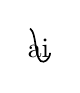
\begin{tikzpicture}[baseline=(letters.base),x=1em,y=1em]
\node[inner sep=0pt] (letters) at (0,0) {ai};
\handwritten{\draw[line width=.6pt] (-.30,.72) .. controls (-.04,.55) and (-.16,-.55) .. (.19,-.48) .. controls (.34,-.46) and (.44,-.22) .. (.42,-.16);}
\end{tikzpicture}l rings\handwritten{''}, prompted by some nice work of Brieskorn on Klein singularities. I very much appreciate this work of yours, and would appreciate getting reprints of any later work you may have available. As I already felt when your work appea\deleted{\unsure{k|r}}\handwritten{r}ed, it cries for careful reconsideration in the framework of \deleted{\unsure{a|A}}\handwritten{A}lg. Geometry, and suggests number of interesting problems. I wonder if you know the answer to some of them. For instance, I feel it would be of interest to classify (for a given complex simple adjoint Lie group, say) quadr\deleted{\unsure{a|u}}uples $(\mathrm{T},\mathrm{B},\mathrm{T}',\mathrm{B}')$, where $\mathrm{T}$ and $\mathrm{T}'$ are maximal tori ``in apposition\handwritten{''} (in your terminology), and $\mathrm{B}$ and $\mathrm{B}'$ Borel subgroups of $\mathrm{G}$ containing $\mathrm{T}$ resp. $\mathrm{T}'$. The number of conjugacy classes of such animals is equal to $\operatorname{card}(\mathrm{W})^{\handwritten{2}}/\mathrm{hz}\handwritten{\phi}(\mathrm{h})$, where $\deleted{\unsure{\mathrm{H}|\mathrm{W}}}\handwritten{W}$ is the Weyl group, $\mathrm{h}$ the Coxeter number, $\mathrm{z}$ the order of the center\inserted{\handwritten{of $\widetilde{G}$}}, and $\handwritten{\phi}(\mathrm{h})=\operatorname{card}(\underline{\mathrm{Z}}/\mathrm{h}\underline{\mathrm{Z}})^{\handwritten{*}}$ is the Euler indicatrix; if you want to classify such data with moreover a\deleted{n} \inserted{\unsure{g\deleted{a}enerating|generating}} element (principal regular in your terminology) given for the finite group of order $\mathrm{h}$ $\mathrm{T}\handwritten{\cap}\mathrm{N}(\mathrm{T}')$, then we get $\operatorname{card}(\mathrm{W})^{\handwritten{2}}/\mathrm{hz}$ choices. One of the reasons I think this question is interesting is that the stablity subgroup in $\mathrm{G}$ of such a quadruple is $\mathrm{T}\handwritten{\cap}\mathrm{T}'=\mathrm{e}$,\handwritten{\textsuperscript{*}} hence such a structure makes $\mathrm{G}$ entirely ``rigid'' up to exterior automorphisms. Among the first questions one may wish to ask in this direction are the following: is it true that for some, or for all, such quadruples, $\mathrm{B}$ and $\mathrm{B}'$ are ``in general position'' i.e. $\mathrm{B}\handwritten{\cap}\mathrm{B}'$ is a torus (necessarily maximal), so that $\mathrm{B}$ and $\mathrm{B}'$ are ``opposite'' to each other with respect to the latter ? Is there in any sense a \uline{distinguished} conjugacy class of such quadruples (which should then be, of course, invariant by action of exterior automorphisms) ? What are the groups of automorph\deleted{k}isms of such quadr\deleted{a}uples (they

\margin{\handwritten{* NB: $N(T)\cap N(T')$ is an extension of $(\mathbb{Z}/h\mathbb{Z})^{*}$ by $\mathbb{Z}/h\mathbb{Z}\times \underset{\substack{\tikz[scale=.2]{\draw (0,0)--(.2,.6);}
\\\text{center of }\widetilde{G}}}{Z}\deleted{\unsure{(G)|(\widetilde{G})}}$, hence of order $hz\varphi(h)$}}
% The short oblique leader and its lower annotation are retained below Z.
% The handwritten transposition stroke crosses the original typed ``ai'' in ``polynomail''; no replacement letters have been supplied.
% archive sheet number: 21

% C123-02_123_scan023
\scanpage{23}
are isomorphic to subgroups of the group of exterior automorphisms of $\mathrm{G}$) ?

In a different direction, it would be\handwritten{\raisebox{.6ex}{$\vert$}}interesting to know more about the canonical morphism $\underline{\mathrm{g}}\handwritten{\longrightarrow}\underline{\mathrm{h}}/\mathrm{W}$, where $\underline{\mathrm{g}}$ is the Lie algebra of $\mathrm{G}$ and $\underline{\mathrm{h}}$ a Cartan subalgebra, and of the orbits of $\mathrm{G}$ on $\underline{\mathrm{g}}$, and the analoguous morphism of Steinberg $\mathrm{G}\handwritten{\longrightarrow}\mathrm{T}/\mathrm{W}$ and the orbits of $\mathrm{G}$ acting on itself. Do you know for instance exactly how varies the rank (= rang of the tangent map) of this \deleted{\unsure{applicati}} map ? There are some reasons to believe that \deleted{this} for points of unipotent orbits of dimension $\inserted{\mathrm{n}-}\mathrm{r}-2$ (just \deleted{the next lower after}\inserted{the next lower after} the maximal dimension $\mathrm{n}-\mathrm{r}$), the rank is $\mathrm{r}-1$ in case all roots have same length (that is the corresponding diagrams $\mathrm{A}_{\deleted{\unsure{\mathrm{n}|\mathrm{r}}}\unsure{\mathrm{r}|\mathrm{n}}},\mathrm{D}_{\deleted{\unsure{\mathrm{n}|\mathrm{r}}}\unsure{\mathrm{r}|\mathrm{n}}},\mathrm{E}_{\handwritten{6}},\mathrm{E}_{\handwritten{7}},\mathrm{E}_{\handwritten{8}}$ are those corresponding to Klein singularities), and $\handwritten{<}\mathrm{r}-1$ in \inserted{\handwritten{all}} other cases; in the first case, I would expect that there is just one orbit as stated, by the way, and maybe this property will be caracteristic of the ``homogene\deleted{\unsure{a|u}}ous'' case when all roots have same length. Also, what can be said of the dim\deleted{\unsure{\$|S}}ension of the set of all Borel subgroups containing a given element $\mathrm{g}\handwritten{\in}\mathrm{G}$, resp. whose Lie algebra contains a given element $\mathrm{x}\handwritten{\in}\underline{\mathrm{g}}$ ? If $2\mathrm{N}=\mathrm{n}-\mathrm{r}$ is the number of roots and if the dimension of the orbit of the given element is $2\mathrm{N}-2\mathrm{i}$, I would expect the dimension of the previous variety to be equal to $\mathrm{i}$; the inequality $\handwritten{\leqslant}\mathrm{i}$ would imply, by generalizing a depth argument of \unsure{Br\deleted{e}i\deleted{i}eskorn|Br\deleted{i}e\deleted{e}iskorn}, that the singularities of the fibers of your map $\underline{\mathrm{g}}\handwritten{\longrightarrow}\underline{\mathrm{h}}/\mathrm{W}$ (resp. Steinberg's $\mathrm{G}\handwritten{\longrightarrow}\mathrm{T}/\mathrm{W}$ in case $\mathrm{G}$ is simply connected instead of adjoint) are ``rational'', i.e. i\deleted{s}f $\mathrm{F}$ is such a fiber and $\mathrm{F}'\overset{\mathrm{f}}{\handwritten{\longrightarrow}}\mathrm{F}$ a resolution of singularities of $\mathrm{F}$, t\deleted{e}h\deleted{h}en $\mathrm{R}^{\mathrm{i}}\mathrm{f}_{\handwritten{*}}(\underline{\mathrm{O}}_{\mathrm{F}'}^{\deleted{\unsure{\mathrm{t}|*}}})=0$ for $\mathrm{i}\handwritten{>}0$. Maybe the ans\deleted{\illegible{1}}w\deleted{\illegible{1}}er \deleted{\unsure{ot|to}}\handwritten{to} most of the questions I am asking are well known and I am just ignorant; for some of them, it would indeed be scandalous that the experts do not know the answer ! In any case, I would be grateful for any comment you would have on any of my questions.

Sincerely yours\\
\handwritten{A\,\unsure{Grothendieck}}\\
% The vertical pen stroke at ``beinteresting'' is retained as a raised bar; no silent space has been supplied.
% archive sheet number: 22
% Isolated non-text vertical mark below the signature; no character reading assigned.

% C123-02_123_scan028
\scanpage{28}
\mspage{\handwritten{\unsure{22|72}}}
% archive sheet number: 27 (inverted at the upper right)
% A single long vertical cancellation stroke runs through the typescript, from the opening paragraph into the footnote. The three enclosing deletion macros preserve this page-wide cancellation; inner deletion macros preserve the local revisions.

\deleted{un morphisme de topos $\mathrm{u}:\mathrm{E}\handwritten{\longrightarrow}\mathrm{E}'$, et ce dernier sera ``unique à isomorphisme unique près'' en termes de la donnée $\mathrm{u}^{\handwritten{*}}$ resp. $\mathrm{u}_{\handwritten{*}}$, en un sens assez clair, et qui sera d'ailleurs entièrement explicité plus bas \handwritten{(\deleted{\unsure{2|3}}3.2.1)}}

\deleted{\deleted{\unsure{2|3}}\handwritten{3}.1.2. Si $\mathrm{u}:\mathrm{E}\handwritten{\longrightarrow}\mathrm{E}'$ est un morphisme de topos, il résulte des propriétés des foncteurs adjoints \inserted{\handwritten{(I 2.11)}} que le foncteur image directe $\mathrm{u}_{\handwritten{*}}:\mathrm{E}\handwritten{\longrightarrow}\mathrm{E}'$ commute aux limites projectives, et le foncteur $\mathrm{u}^{\handwritten{*}}:\mathrm{E}'\handwritten{\longrightarrow}\mathrm{E}$ commute aux limites inductives \deleted{\unsure{(2.11)|(2.1)|(I 2.11)}}\handwritten{(${}^{*}$)}.Comme on suppose de plus que ce dernier \inserted{\handwritten{est \unsure{exact|ex.ct} à gauche i.e.}} commute aux limites projectives finies, on voit donc en particulier que $\mathrm{u}^{\handwritten{*}}$ \uline{est} \deleted{exac} \uline{exact}. \inserted{On peut donc dire que} \uline{\deleted{C}\handwritten{c}'est \deleted{donc} le foncteur image inverse} $\mathrm{u}^{\handwritten{*}}$ \deleted{qui}, dans le couple $(\mathrm{u}_{\handwritten{*}},\mathrm{u}^{\handwritten{*}})$, \uline{qui possède les propriétés d'exactitude les plus remarquables}, \deleted{assurant} Ces propriétés assurent que pour toute espèce de structure algébrique \inserted{\handwritten{$\Sigma$}}\deleted{qui peut} dont les données peuvent se décrire en termes de données de flèches entre les ensembles de base et des ensembles déduits de ceux-ci par application répétée d'opérations de limites projectives finies et de limites inductives quelconques, \inserted{\handwritten{et pour}} tout \handwritten{``}objet de $\underline{\mathrm{E}}'$ muni d'une structure d'espèce $\handwritten{\Sigma}$'' (notion qui a un sens grâce aux propriétés d'exactitude \deleted{de} internes du topos $\unsure{\mathbb{E}'|\underline{\mathrm{E}}'}$ (II 4.1)), son image \deleted{inverse} par $\mathrm{u}^{\handwritten{*}}$ est muni des mêmes structures. Plutôt que d'entrer dans la tâche peu engageante de donner un sens précis à cet énoncé et de le justifier de façon formelle, nous conseillons au lecteur de \inserted{l'expliciter et de} se convaincre de sa validité pour des espèces de structure telles que celle de groupe, d'anneau, de module sur un anneau, de comodule \deleted{ou de bimodule} sur un anneau, de bigèbre sur un anneau, de torseur sous un groupe. (Dans ces exemples, les trois premières espèces de structure se définis}
% The last word is cut at the right image edge after the visible fragment ``définis''; no unseen ending is supplied. The parenthesis is open on the source page.

% Left margin beside the body reference on L07.
\margin{\handwritten{\deleted{\unsure{(I 2.11)|(I 4.11)|(I 4.1)}}.}}

\handwritten{\figure{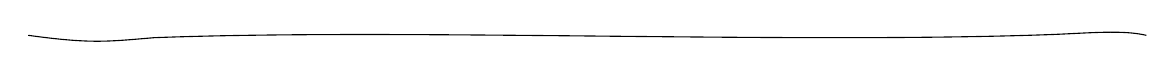
\begin{tikzpicture}[x=1cm,y=1cm]
\draw[line width=.4pt] (0,.03) .. controls (.8,-.08) and (1.0,-.05) .. (1.6,0) .. controls (4.8,.12) and (9.7,-.08) .. (13.0,.04) .. controls (13.5,.06) and (13.9,.10) .. (14.2,.03);
\end{tikzpicture}}}

\deleted{($\handwritten{*}$) \deleted{On peut} \deleted{d}\handwritten{D}'ailleurs \deleted{vérifier que}\inserted{\handwritten{(1.5 et 1.8)}}, pour un foncteur $\mathrm{u}_{\handwritten{*}}:\mathrm{E}\handwritten{\longrightarrow}\mathrm{E}'$ resp. $\mathrm{u}^{\handwritten{*}}:\mathrm{E}'\handwritten{\longrightarrow}\mathrm{E}$ donné, \deleted{\unsure{d}}\handwritten{c}e foncteur admet un adjoint à gauche (resp. à droite si et seulement si il commute aux \inserted{$\underline{\mathrm{U}}$-}limites projectives (resp. aux $\underline{\mathrm{U}}$-limites inductives). \deleted{\unsure{D'ailleurs}, c'est une conséquence immédiate de 1.2.\unsure{(ii)|(iii)|(i)}}}
% The right edge after ``droite'' is cropped; no unseen closing parenthesis has been added.

% C123-02_123_scan040
\scanpage{40}
\mspage{\handwritten{23}}
% archive sheet number: 39 (inverted, upper left)
% The two loop-and-stem signs below reproduce the handwritten linking marks; they are not read as letters.
% The top and bottom marginal continuations are placed at their marked insertion points.
sent en termes de limites projectives finies exclusivement, tandis que les autres notions impliquent implicitement des constructions faisant appel également à des limites ind\unsure{\deleted{c}u|u}\unsure{\deleted{u}c|c}tive\unsure{\deleted{s}s|s})\handwritten{)}.
\inserted{\handwritten{De plus, le foncteur $u^{*}$ ``\uline{commute}'' à toutes
\tikz[baseline=-0.3ex,scale=.18]{\draw (0,1.3)--(0,.15) .. controls (-.4,-.2) and (.4,-.2) .. (0,.15);}
\figure{\begin{tikzpicture}
\node[inner sep=6pt,text width=.88\linewidth,align=left] (n) {\tikz[baseline=-0.3ex,scale=.18]{\draw (0,1.3)--(0,.15) .. controls (-.4,-.2) and (.4,-.2) .. (0,.15);}les opérations fonctorielles \deleted{\illegible{1}} habituelles faites en termes de telles structures, plus précisément à toutes les opérations qui \inserted{peuvent} s'exprime\deleted{nt}\unsure{r} en termes de $\varinjlim$ et de $\varprojlim$ finies: constructions d'objets libres (groupes ou modules libres, p.ex.) engendrés par un objet, produits tensoriels (cf. \S 6 plus bas) etc.};
\draw ([yshift=2mm]n.north west) .. controls ([xshift=-2mm]n.west) and ([xshift=-1mm]n.south west) .. (n.south west) -- ([xshift=1mm]n.south) -- ([xshift=2mm,yshift=2mm]n.south) -- ([yshift=2mm]n.south east);
\end{tikzpicture}}}}

\margin{\handwritten{\figure{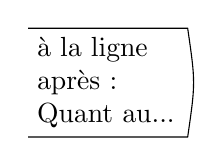
\begin{tikzpicture}\node[align=left,text width=1.8cm,inner sep=3pt] (n) {à la ligne après : Quant au...};\draw (n.north west)--(n.north east) .. controls ([xshift=1mm]n.east) .. (n.south east)--(n.south west);\end{tikzpicture}}}}
% The opposing pen brackets mark the paragraph break immediately before Quant au.
\handwritten{\tikz[baseline=-.6ex,scale=.18]{\draw (0,1.5)--(.5,1.4)--(.6,0)--(0,-.15);\draw (1.4,1.4)--(.9,1.35)--(.9,-.1)--(1.5,-.15);}}
Quant au foncteur image directe $\mathrm{u}_{\handwritten{*}}$\inserted{$:\mathrm{E}\handwritten{\longrightarrow}\mathrm{E}'$}, qui commute aux limites projectives, il ``respecte'' \inserted{par suite} toute structure algébrique sur un objet (ou une famille d'objets) de $\mathrm{E}$, définissable en termes de limites projectives \inserted{exclusivement} (telles les str\deleted{i}uctures de groupe, d'anneau ou de module sur un anneau, \deleted{dans}\inserted{parmi} les exemples précédents). Par \deleted{f}contre, le foncteur $\mathrm{u}_{\handwritten{*}}$ n\deleted{e}'est en général pas exact à droite i.e. il ne commute pas en général aux limites inductives finies, et même ne transforme pas en général épimorphisme en épimorphisme\handwritten{\unsure{;|,}} (c'est d'ailleurs \deleted{\unsure{comme} nous le verrons au} ce défaut d'exactitude du foncteur $\mathrm{u}_{\handwritten{*}}$ qui est \handwritten{à} la source de ces propriétés cohomologiques, qui seront étudiées (du point de vue de l'algèbre homologique commutative) dans l'exposé suivant\handwritten{)}.
\inserted{\handwritten{Par suite, il ne \deleted{transforme pas}\inserted{s'étend pas}, en général,
\tikz[baseline=-.3ex,scale=.18]{\draw (0,0)--(.05,1.3) .. controls (-.35,1.65) and (.45,1.65) .. (.05,1.3);}
\figure{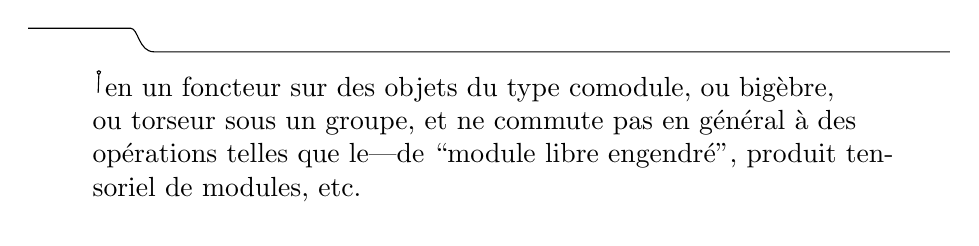
\begin{tikzpicture}
\node[inner sep=6pt,text width=.88\linewidth,align=left] (n) {\tikz[baseline=-.3ex,scale=.18]{\draw (0,0)--(.05,1.3) .. controls (-.35,1.65) and (.45,1.65) .. (.05,1.3);}en un foncteur sur des objets du type comodule, ou bigèbre, ou torseur sous un groupe, et ne commute pas en général à des opérations telles que \deleted{\unsure{le|de}} ``module libre engendré'', produit tensoriel de modules, etc.};
\draw ([xshift=-6mm,yshift=3mm]n.north west)--([xshift=7mm,yshift=3mm]n.north west) .. controls ([xshift=8mm,yshift=3mm]n.north west) and ([xshift=8mm]n.north west) .. ([xshift=10mm]n.north west)--(n.north east);
\end{tikzpicture}}}}

\deleted{2}\handwritten{3}.1.\handwritten{3}. En pratique, lorsqu'on \deleted{se donne}\inserted{est \inserted{\handwritten{en}} présenced'}un foncteur $\mathrm{f}:\mathrm{E}\handwritten{\longrightarrow}\mathrm{F}$ d'un $\underline{\mathrm{U}}$-topos dans un autre, il y a lieu d'en expliciter \inserted{\handwritten{toutes}} les propri\deleted{t}é\deleted{é}tés d'exactitude, \deleted{y compris et de déterminer s'il admet un foncteur exact} y compris l'existence éventuelle de foncteurs adjoints à gauche ou à droite (cf. la note de bas de page précédente), pour parvenir à une compréhension de la ``nature géométrique'' de $\mathrm{f}$, \deleted{qui} compréhension qui sera généralement un guide indispensable pour \deleted{l'}\inserted{une}intuition géométrique correcte de la situation. Ainsi, s'il s'avère que $\mathrm{f}$ commute aux limites inductives quelconques et aux limites projectives finies, il y a lieu d'écrire $\mathrm{f}$ sous la forme
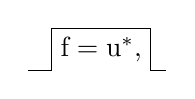
\begin{tikzpicture}[baseline=(n.base)]\node[inner sep=3pt] (n) {$\mathrm{f}=\mathrm{u}^{\handwritten{*}}$,};\handwritten{\draw ([xshift=-3mm]n.south west)--(n.south west)--(n.north west)--(n.north east)--(n.south east)--([xshift=2mm]n.south east);}\end{tikzpicture}
où
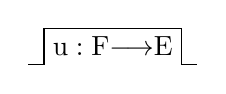
\begin{tikzpicture}[baseline=(n.base)]\node[inner sep=3pt] (n) {$\mathrm{u}:\mathrm{F}\handwritten{\longrightarrow}\mathrm{E}$};\handwritten{\draw ([xshift=-2mm]n.south west)--(n.south west)--(n.north west)--(n.north east)--(n.south east)--([xshift=2mm]n.south east);}\end{tikzpicture}
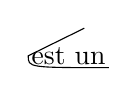
\begin{tikzpicture}[baseline=(n.base)]\node[inner sep=1pt] (n) {est un};\handwritten{\draw ([xshift=2mm,yshift=2mm]n.north)--(n.west) .. controls (n.south west) .. (n.south east);}\end{tikzpicture}
morphisme de topos, i.e. d'interpréter $\mathrm{f}$ comme un foncteur ``image inverse'' par une ````application continue'' de topos. Lorsque $\mathrm{f}$ commute aux limites projectives quelconques, donc qu'il admet un adjoint à gauche,\deleted{$\mathrm{g}$}

\cotefile{162-1}

% H162-01_162-1_scan002
\scanpage{2}
\noindent\hfill Papiers prêtés

\margin{$\overline{\underline{\mathrm{III}}}$}

\margin{(\unsure{8|8.} \unsure{p|p.})}

% isolated oblique ink stroke at right, without textual attachment or a securely legible character

% archive sheet number: 1

\clearpage

% H162-01_162-1_scan004
\scanpage{4}
Raynaud\qquad Mumford . $\Theta$ \unsure{function|fonction} \textcircled{\scriptsize $\overline{\underline{\mathrm I}}$}, $\overline{\underline{\mathrm{II}}}$

Papiers Kiehl

\unsure{Artin}-Winters

Illusie 1\qquad Monsky-Washnitzer $\overline{\underline{\mathrm{I}}},\overline{\underline{\mathrm{II}}}$

/\quad lettres Hartshorne

Hartshorne : Affine duality

/\quad Lettres Quillen

Notes sur extensions \unsure{infinitésimales}

\deleted{Notes sur \unsure{tapis|topis|topos} (\unsure{pluriel|Gabriel}) Quillen}

Rapport Bourbaki calcul différentiel

Complexe cot$_{\unsure{*|+}}$ relatif de Quillen

Notes sur L'extension d'Atiyah \unsure{pour|par} $\Omega^{1}$ ..---

Koszul\quad 2 articles

\deleted{\unsure{Borel}\qquad Lecture Notes}

\figure{\begin{tikzpicture}
\draw[line width=.3pt] (0,0) .. controls (1.2,-.05) and (2.9,.13) .. (4.35,.17);
\draw[line width=.25pt] (4.52,.19) .. controls (5.5,.13) and (6.9,.26) .. (8.05,.30);
\end{tikzpicture}}

Deligne \unsure{1|2|?}\qquad Monsky-Washnitzer

\deleted{(\unsure{suite|suiten})}

\deleted{\uuline{Serre} : Ch. Vect. Witt et var. abéliennes en car $p\ne0$.}

Preprint Griffiths : ``On monodromy ....''

\deleted{Lettre \uwave{\unsure{Rietzly|Rietzley} Chapin}, \unsure{class} field th\unsure{y|.}}

\deleted{\unsure{Qui|Que}}

\deleted{Weil : Jacobiennes \unsure{intermédiaires}.}

\deleted{Papiers d'Artin (\uuline{13})}

\deleted{Lichtenbaum, surfaces \unsure{arithmétiques}}

\deleted{Manin, variétés rationnelles (2 articles)}

\deleted{\unsure{Harder|Hardy} sur conjecture de Weil}

% archive sheet number: 3

\clearpage
